\prefacesection{Regular Expression Parser}
The following report with describe a regular expression parser along with it's design and implementation. The parser shall take a given input and do an analysis of regular expressions. This report will consist of three parts. Firstly. A section of the lexical categories will be brought forward to discuss the architecture of the lexicon. A section on the implementation will be provided to describe the program being developed and how it interacts with the lexical entries. Lastly, a system architectures section will state the issues that were encountered during the process of development and how they were resolved. A conclusion will be given to summarize the points made during the report. Additionally, the project will be developed with Java and the report shall be with LaTeX.

\section*{Lexical Categories}
Firstly, the lexical categories are ordered from the sentence of \textit{The/a man/men/woman/women bite(s)/like(s) the green dog}. Each word was specified with a part-of-speech category and a number (Singular or plural). Each abbreviation for the POS categories are taken in accordance of the results from the Stanford CoreNLP library. The categories are as follows:
\newpage
\begin{itemize}
	\item Determiner - \textbf{DT}
	\item Common Noun - \textbf{NN}
	\item Noun Plural Form - \textbf{NNS}
	\item Verb Base Form - \textbf{VB}
	\item Verb 3rd Person Singular - \textbf{ VBZ}
	\item Adjectives - \textbf{JJ}
\end{itemize}
Therefore, the structure of the lexicon and it's parts-of-speech can be seen in table below.


\begin{longtable}{|c|p{2cm}|c|c|c|}
	\hline 
	\textbf{Word}
	& \textbf{POS}
	& \textbf{Number}
	\\ 
	\hline 
	The & DT & Singular \\ 
	\hline 
	A  & DT & Singular \\ 
	\hline 
	Man & NN & Singular \\ 
	\hline 
	Men & NNS & Plural \\ 
	\hline 
	Woman & NN & Singular \\ 
	\hline 
	Women & NNS & Plural \\ 
	\hline 
	Bite & VB & Singular \\ 
	\hline 
	Bites & VBZ & Singular \\ 
	\hline 
	Like & VB & Singular \\ 
	\hline 
	Likes & VBZ & Singular \\ 
	\hline 
	Green & JJ & Singular \\ 
	\hline 
	Dog & NN  & Singular \\ 
	\hline 
\end{longtable}




% e.g. noun, verb etc. in terms of the architecture of the lexicon


\section*{Implementation}
% describing how you have implemented your parser program and its interface to the lexicon and how it uses the lexical entries.  

Initially, the parser program takes the input entered by the user. The input is then tokenized. These tokens are traversed to in while loop. Additionally, the lexicon file is scanned using the \textit{java.util.Scanner} class. Each line from the lexicon is also tokenized for evaluation. Within each token of the users input, the file is searched to determine wether the word is contained within the lexicon. If the word is found in the file, the second token (which is the part-of-speech tag) is added to an array list. This is done for all tokens in the users input. Following this, the array list is traversed and concatenated to a string. This string is then compared to a structure expected for it to be an acceptable regular expression. The result is then printed to the user interface. This can be seen in Figure 1.

\begin{figure}[ht]
	\begin{center}
		\advance\leftskip-3cm
		\advance\rightskip-3cm
		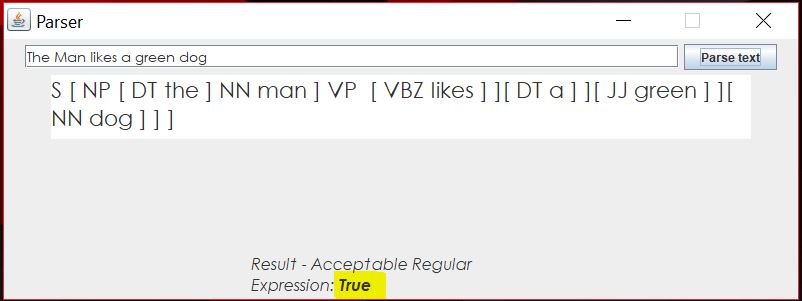
\includegraphics[keepaspectratio=true,scale=0.9]{__resources/true.jpg}
		\caption{Result For Acceptable Input}
		\label{onset}
	\end{center}
\end{figure}

Additionally, if a text is entered that does meet match the words used in the lexicon, or that is in the wrong order, the user interface is updated to display that it is not a suitable regular expression. This is displayed in Figure 2.

\begin{figure}[ht]
	\begin{center}
		\advance\leftskip-3cm
		\advance\rightskip-3cm
		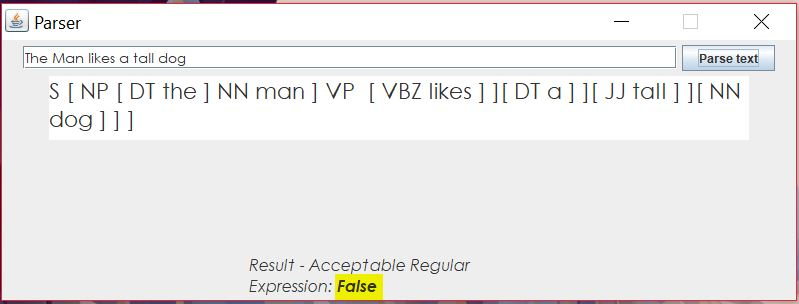
\includegraphics[keepaspectratio=true,scale=0.9]{__resources/false.jpg}
		\caption{Result For Non-acceptable Input}
		\label{onset}
	\end{center}
\end{figure}


\section*{System Architecture}
%providing a description of your software design stating the problems that you needed to address and how you surmounted them... for each of these, state individually the problem and then your solution.  

\textbf{Parser}\\
The program's initial state is to display the user interface. As seen in Figure 1 and Figure 2, the view consists of a JTextField for the users input. A JTextArea can be seen beneath which displayed the users input in the bracket phrasal structure. This is performed by the \textbf{PrintBracket} Class, which checks the users input and print the POS tags and words entered. The interface also includes a button which calls \textbf{ParserButtonListener} when clicked for parsing the user input. At the bottom of the user interface a result is displayed, which is changed by the \textbf{ValidateInput} class. Each of the interactive components are static types so they may be modified by other classes.\\ \\
\textbf{ParserButtonListener} \\
This class implements the ActionListener interface to react to a users interaction with the "Parse Text" button. When clicked, the text from the input field is taken and converted to lower case characters. The string is tokenized into tokens for validation of an acceptable regular expression. Additionally, the string is tagged using the Stanford CoreNLP library. 
A ValidateInput and a PrintBracket object are created and the inputs are passed accordingly to each object to update the user interface and validate the input string. Initially, the validation and the output display were done within the same class, but this ran into problems when ever an input that did not satisfy the regular expression as it would only print the words that were found in the lexicon. Therefore, in order to get around this, the user input was validated and formatted for the bracket structure separately. \\ \\
\textbf{ValidateInput}\\
This class is used to evaluate the string entered by the user and determine if it is valid or not. The tokenized input is passed as a parameter in the validate() method and traversed in a while loop. Each token is then compared to the tokenized lexicon entries by line to see if the word is part of the systems lexicon. If it is, the words POS tag (second token in the \textbf{lexiconTokens} tokens) is added to a categories array list. After all tokens are traversed, the array list is converted to a string and evaluated if the parts-of-speech meet the requirements to be an acceptable expression. If all tags are met, then the result is displayed as \textbf{true}, other it is \textbf{false}. See code below.

\begin{lstlisting}
	if(posTags.equals("DT NN VBZ DT JJ NN ") ||
	   posTags.equals("DT NNS IN DT JJ NN ") ||
	   posTags.equals("DT NNS VBZ DT JJ NN ") ||
	   posTags.equals("DT NN IN DT JJ NN ")){
		
	   Parser.acceptable.setText("<html>Result - Acceptable 
	   Regular Expression: <b>True</b></html>" );
	}
	else{
	   Parser.acceptable.setText("<html>Result - Acceptable 
	   Regular Expression: <b>False</b></html>" );
	}
\end{lstlisting}\\ \\ 
\textbf{PrintBracket}\\
In this class, the used input is also tokenized and traversed with a while loop. In this loop two strings are made using regular expression to separate the tag from the tokenized input from the user. This is done because the output for each token from the Stanford CoreNLP library results in a \textbf{word\_TAG} format. For example, if the word "dog" was entered, the tagged value is "dog\_NN".  See code below.
\begin{lstlisting}
	while(taggedTokens.hasMoreTokens()){
 	  String t = taggedTokens.nextToken();
	  String s = t;
	  t= t.replaceAll("[a-z]+_", "");
	  s =s.replaceAll("_[A-Z]+", "");
	  posTags.add(t);
	  words.add(s);
	}
\end{lstlisting}
The words and tags are added to their own respective array list. After all tokens are properly separated, the then evaluated to be printed into a bracket phrasal structure. This is done by checking the size of the POS tag array list to give a pedicted structure output. For further illustration of the system architecture, please refer to the UML diagram displayed in Figure 3.
\begin{figure}[ht]
	\begin{center}
		\advance\leftskip-3cm
		\advance\rightskip-3cm
		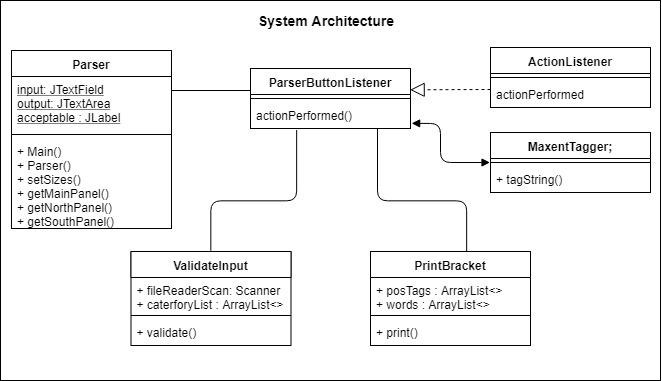
\includegraphics[keepaspectratio=true,scale=0.5]{__resources/uml.jpg}
		\caption{Result For Non-acceptable Input}
		\label{onset}
	\end{center}
\end{figure}

\section*{Conclusion}
In conclusion, the program was able to take a users input, print a bracketed phrasal structure output to the user interface even if the the input was a valid regular expression or not, and was able to validate the input of the user in accordance to the sentence specified in the requirements.
